\chapter{Metodo dei due grafi}

\section{Teoria}

Il metodo dei due grafi è ad oggi forse la tecnica più performante per la risoluzione del problema dell'analisi simbolica. Questo metodo si appoggia alla rappresentazione di un circuito elettrico tramite l'uso di due grafi detti \textbf{Grafo in Corrente (gI)} e \textbf{Grafo in Tensione (gV)}. Come visto in precedenza, i due grafi ottenuti dalla sintesi dei componenti presenti nel circuito hanno stessa cardinalità per quanto riguarda l'insieme dei nodi e quello degli archi. Se si considera inoltre il processo di costruzione adottato, si possono trarre interessanti conclusioni:
\begin{itemize}
 \item I grafi \textit{gI} e \textit{gV} hanno, appunto, uno stesso numero di nodi e uno stesso numero di archi
 \item Un albero per \textit{gI} ha lo stesso numero di archi di un albero per \textit{gV} e viceversa, pari al numero di nodi diminuito di uno
 \item Per costruzione, laddove l'$i_{esimo}$ arco di \textit{gI} si riferisca ad un componente $C$, allora anche l'$i_{esimo}$ arco di \textit{gV} si riferirà a quello stesso componente (questo perché i componenti introducono uno stesso numero di archi in ogni grafo e si suppone che gli archi vengano etichettati in base all'ordine di inserimento)
\end{itemize}
Nota: dall'ultimo punto si deduce che le informazioni non necessitano di essere duplicate, bensì condivise fra i singoli archi che si corrispondono nei due grafi, il che contribuisce ad abbattere ulteriormente lo spazio richiesto per la memorizzazione.

Molto importante, pertanto degno di essere ribadito ancora una volta, è il fatto che gli archi debbano essere etichettati, immagazzinati o comunque recuperabili nello stesso ordine di immissione. Su questo punto, infatti, si basa l'intero algoritmo che sarà illustrato di seguito e questo stesso aspetto rappresenta spesso un approccio scarsamente considerato nell'uso di grafi. Osservando la questione dal punto di vista opposto, si può formulare un enunciato come segue:

\paragraph{}
\emph{
Siano $gI^L$ e $gV^L$ due liste di archi aventi stessa cardinalità e sulle quali sia indotto un ordinamento (ad esempio basato sulla posizione occupata nella lista), supposto che gli archi siano definiti su uno spazio di vertici avente cardinalità $N$ in entrambi i casi, allora si ha che:
\begin{itemize}
 \item Le due liste concorrono a definire due grafi distinti, \textit{gI} e \textit{gV}, composti rispettivamente dai due elenchi di archi, aventi stessa cardinalità tanto in numero di vertici quanto in numero di archi.
 \item Un albero comune è dato da un insieme di indici $I^T$ di cardinalità $N-1$ tale che, sfruttando gli ordinamenti indotti sulle due liste, gli archi individuati da tali indici in ognuna di esse descrivono un albero sul grafo corrispondente.
 \item Un insieme di indici $I^E$ di cardinalità $N-1$ tale che gli archi individuati nelle due liste formano solamente in uno dei due casi un albero per il grafo corrispondente, non si può definire tale da descrivere un albero comune
\end{itemize}
}

\paragraph{}

\begin{figure}[b]
 \centering
 \subfloat[Grafo in corrente]{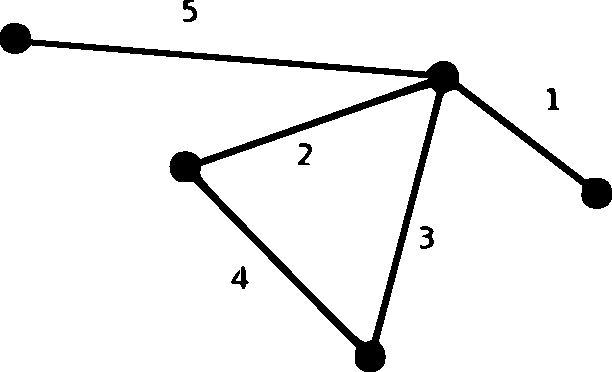
\includegraphics[scale=0.5]{immagini/gi.pdf}}
 \hspace{25pt}
 \subfloat[Grafo in tensione]{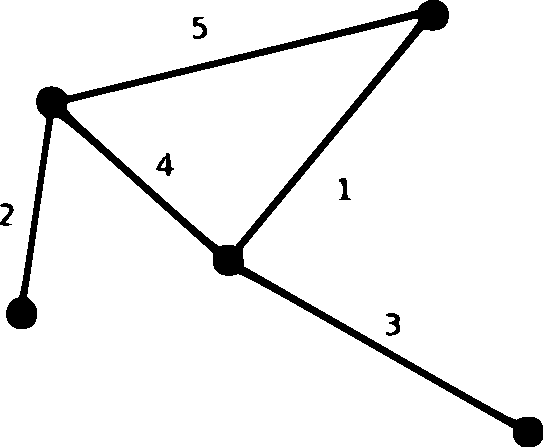
\includegraphics[scale=0.5]{immagini/gv.pdf}}
 \caption{Coppia di grafi con alberi in comune}
 \label{fig:gigv}
\end{figure}

Data la semplicità del concetto ma la sua difficoltà di esposizione, si procede con un esempio. Osserviamo la figura \ref{fig:gigv}, dove sono descritti due grafi che possono essere derivati dalla sintesi di un circuito elettrico. Gli archi sono numerati, per costruzione, in base all'ordine di immissione e pertanto l'arco $1$ nel primo e nel secondo grafo sarà legato allo stesso pacchetto di informazioni esterne all'algoritmo di ricerca degli alberi comuni. Cambiando punto di vista, se l'informazione viene scelta, ciò implica che i due archi etichettati con $1$ vengono scelti.\\
Con una semplice occhiata si nota che i due grafi hanno almeno un albero in comune, dato dagli archi etichettati con $1-2-3-5$. Dalle ipotesi sopra, restituendo questo insieme di indici al richiedente, sarà sufficiente accedere ai blocchi di dati legati al singolo indice per recuperare le informazioni necessarie, senza dovere ulteriormente interagire con la coppia di grafi che (a parte l'etichetta associata al singolo arco) niente sanno delle informazioni presenti.

\paragraph{}
Riassumendo, quindi, l'idea è quella di costruire in maniera idonea i due grafi, così che si possano dare in pasto ad un algoritmo di ricerca degli alberi comuni che non debba preoccuparsi dei dati legati ai singoli archi, poiché a priori non ci sono riserve sull'inclusione o esclusione di una coppia di archi legati fra loro. Su tali presupposti si può quindi operare ottenendo una lista di alberi in comune a partire dalla quale, in seguito, sarà estrapolata la soluzione cercata con tecniche apposite che esulano dall'obiettivo dell'algoritmo di ricerca.\\
Di seguito verranno illustrati due algoritmi, uno il miglioramento dell'altro, che mirano appunto a individuare alberi in comune fra grafi descritti come lista di archi, pertanto è compito dell'utente costruire in maniera attenta tale lista.



\section{Il metodo di Grimbleby}

Questo primo metodo è descritto in \cite{Grimbleby} e, sebbene sia stato usato largamente e per molti anni (anche e soprattutto in Sapec), soffre di alcune carenze dal punto di vista dell'ottimizzazione. Come vedremo in seguito, infatti, con pochi semplici accorgimenti si può evitare di percorrere alcune strade che si rivelano a priori sterili, alla ricerca di alberi in comune.\\
Ciò nonostante, per quello che ha rappresentato nel campo dell'analisi simbolica, l'algoritmo di Grimbleby deve essere introdotto, poiché ha il merito di definire una base di partenza per lo sviluppo di molte altre metodologie più performanti.

L'algoritmo di Grimbleby\graffito{Il metodo di Grimbleby prende il nome dal suo autore, James B. Grimbleby, e si basa sui risultati ottenuti da Nicos Christofides nel campo della teoria dei grafi} è stato concepito in seno al problema dell'analisi simbolica e quindi costruito sulle ipotesi sopra elencate, per quanto riguarda i due elenchi di archi. Parte cioè dal presupposto che siano definiti due grafi (di tensione e di corrente) aventi stesso numero di nodi e stesso numero di archi e tali che su questi ultimi sia indotto un ordinamento di qualche genere. Il metodo è basato sull'algoritmo di ricerca di un albero di copertura per un grafo come descritto in \cite{GraphTheory} che, come indicato anche dall'autore stesso, è probabilmente inferiore in termini di prestazioni rispetto ad altri algoritmi. Di seguito è riportato l'algoritmo proposto originale, corredato di alcune condizioni a monte e alcune note sulle strutture dati.

\paragraph{}
\emph{
Supponiamo di avere due grafi, $G1$ e $G2$, composti da $N$ nodi e $M$ archi. Inoltre, supponiamo di poterci appoggiare a due grafi inizialmente costituiti dai soli vertici e privi di archi (grafi di questo tipo vengono detti anche foreste), chiamati $H1$ e $H2$. Infine, si utilizzerà uno stack $S$ di capacità pari a $N-1$ ed un contatore $K$ (quest'ultimo è indicato come \textit{puntatore ad arco}, nel senso che mantiene l'indice di riferimento dell'arco in esame). L'algoritmo si sviluppa in pochi semplici passi ed è facilmente implementabile come macchina a stati (tecnica seguita in SapecNG):
\begin{enumerate}
 \item \textbf{Inizializzazione:} $H1$ e $H2$ non contengono inizialmente archi e sono considerati come foreste di $N$ alberi (in altre parole, ogni arco non connesso è considerato un albero e così lo sarà anche nel seguito), lo stack è svuotato e $K$ è posto a $0$.
 \item \textbf{Controllo per albero comune:} se nello stack sono presenti $N-1$ archi, allora è stato individuato un albero comune; gestirlo (o memorizzarlo) e passare al punto 7.
 \item \textbf{Selezione di un nuovo arco:} Incrementare $K$ ($K = K+1$); se non vi è un numero sufficiente di archi per completare un albero (ovvero, $size(stack) + M - K < N - 2$) passare al punto 6.
 \item \textbf{Controllo generazione ciclo:} se l'arco $K$ di $G1$ ($G2$) genera un ciclo in $H1$ ($H2$), allora passare al punto 3.
 \item \textbf{Inclusione arco:} porre $K$ in cima allo stack, quindi includere l'arco $K$ di $G1$ ($G2$) in $H1$ ($H2$). Sia in $H1$ che in $H2$ questo comporterà la fusione di due alberi in uno solo.
 \item \textbf{Controllo completamento:} se lo stack è vuoto, l'algoritmo è concluso e tutti gli alberi di copertura comuni sono stati individuati e gestiti o memorizzati.
 \item \textbf{Backtrack:} rimuovere un arco dalla cima dello stack $S$, quindi porre $K$ pari ad esso; rimuovere l'arco $K$ di $G1$ ($G2)$ da $H1$ ($H2$), il che concorrerà a suddividere in $H1$ ($H2$) un singolo albero in due alberi distinti. Passare al punto 3.
\end{enumerate}
}

\paragraph{}
I grafi $G1$ e $G2$ non richiedono una particolare struttura dati e viene consigliato un immagazzinamento sotto forma di due liste di $M$ coppie di nodi. Per quanto riguarda $H1$ e $H2$, invece, è consigliata l'individuazione di una struttura dati che faciliti le seguenti operazioni:
\begin{itemize}
 \item Controllo nel caso in cui un particolare arco (quando aggiunto in $H1$ o $H2$) generi un ciclo; ciò è equivalente a controllare dove i due archi componenti appartengono già ad uno stesso albero.
 \item Inclusione di un arco con conseguente connessione di due alberi, quindi fusione di questi ultimi in un singolo albero.
 \item Rimozione di un arco, quindi scissione di un albero in due alberi distinti.
\end{itemize}
In \cite{Grimbleby} è proposta la soluzione descritta di seguito. Si crei una lista di cardinalità $N$ per ognuno dei grafi, i cui componenti sono coppie di puntatori:
$$(R_j, P_j), \forall j=1\dots N$$
In ogni albero del grafo un vertice è scelto in modo arbitrario per essere il nodo radice: $R_j$ è la radice dell'albero a cui il nodo $j$ appartiene, mentre $P_j$ è il diretto antenato del nodo $j$ ed è tale che la coppia $(j, P_j)$ rappresenti un arco valido (i nodi radice sono eccezioni e non hanno antenati, in altri termini si può porre come loro antenato sé stessi). Tale lista di $N$ coppie radice e antenato definisce completamente il grafo e si presta in modo particolare ad essere maneggiata facilmente sulla base delle richieste fatte in precedenza.

Inizialmente poiché $H1$ e $H2$ non contengono archi e ogni vertice è considerato un albero a sé stante, ogni nodo è la propria radice e non ha predecessori, ovvero:
$$ \forall j=1\dots N : R_j = j, P_j = 0 $$
Quindi, i tre punti di cui sopra si risolvono banalmente come segue:
\begin{itemize}
 \item La generazione di un ciclo durante l'aggiunta di un arco $(i, j)$ può essere individuata semplicemente controllando se $R_i$ e $R_j$ hanno uno stesso valore, poiché se così fosse allora si può dedurre che $i$ e $j$ appartengano ad uno stesso albero. Segue che l'aggiunta dell'arco $(i, j)$ genererà inevitabilmente un ciclo.
 \item L'inclusione di un arco $(i, j)$ e quindi la fusione di due alberi in uno solo richiede:
           \begin{description}
            \item[Modifica radici sui vertici] Tutti i nodi con radice $R_j$ la vedano cambiata in $R_i$.
            \item[Modifica radice sull'albero] Gli antenati sul cammino fra $j$ e $R_j$ vengano ribaltati, questo renderà $j$ radice dell'albero.
            \item[Modifica antenato] $P_j$ venga cambiato in $i$.
           \end{description}
 \item La rimozione di un arco $(i, j)$ e quindi la scissione di un albero in due alberi distinti richiede:
           \begin{description}
            \item[Normalizzazione indici] Siano scambiati $i$ e $j$ laddove $P_j \neq i$, così che si abbia $P_j = i$.
            \item[Scissione] Siano posti $P_j = 0$ e $R_j = j$, ovvero $j$ diventi la radice dell'albero disconnesso.
            \item[Correzione radici] Considerando ogni nodo $l$ in $\{ 1\dots N\}$ ad eccezione di $j$, se $R_l \neq j$ e $R_{P_l} = j$ allora si ponga $R_l = j$. Questo passo deve essere ripetuto sui vertici fintanto che avvengono modifiche sulle radici.
           \end{description}
\end{itemize}

\paragraph{}
Nonostante gli sforzi per proporre strutture dati idonee, l'algoritmo di Grimbleby soffre come già anticipato di una grave mancanza: un controllo aprioristico che gli permetta di potare i rami del proprio cammino evitando di percorrere strade sterili. Ciò lo rende notevolmente meno performante di quello incluso in QSapecNG che, per onor di cronaca, è concepito a partire da quello sopra proposto che appunto funge da base e punto di partenza per questa branca di algoritmi su grafi. 

Una implementazione in C per SapecNG dell'algoritmo di Grimbleby esiste ed è pensata come macchina a stati, poiché per la sua struttura ed esposizione si presta in maniera particolare. Le richieste in termini di occupazione di memoria per le proprie strutture dati non sono esose, sebbene mantenere due grafi paralleli ($H1$ e $H2$) per facilitare la costruzione degli alberi possa incidere notevolmente sul conto finale, soprattutto nel caso in cui si affrontino grafi $G1$ e $G2$ di dimensioni molto grandi (come è plausibile aspettarsi, un po' perché dimensioni piccole indicano un circuito associato molto piccolo, che quindi non ha bisogno di un software apposito per essere studiato e un po' perché molti componenti includono più di un arco in ognuno dei due grafi, il che ne facilita l'esplosione).

In \cite{Schach} viene fatta un'analisi di tale algoritmo e viene dimostrato come, ad esempio, se ne possano aumentare le performance fino al 50\% semplicemente utilizzando una struttura dati doppiamente collegata tramite puntatori per la memorizzazione degli alberi, il che rende facilmente un'idea delle lacune del metodo di Grimbleby.


\section{Il metodo di Schach}

Questo secondo metodo si sviluppa a partire dall'algoritmo di Grimbleby e viene descritto nel dettaglio in \cite{MRT}. Del suo predecessore eredita gli spunti più interessanti e l'idea di fondo, aggiungendo alcune tecniche che limitino le richieste di occupazione per le strutture dati e che siano in grado di prevenire la ricerca di alberi su percorsi che si possono individuare come sterili a priori. Alla base vi è il riconoscimento che l'algoritmo di Grimbleby si basa completamente su un metodo inefficiente \cite{GraphTheory} e quindi già di partenza ha un corredo di svantaggi in eredità. Come conseguenza nel caso peggiore si ha la generazione di un numero altissimo di plausibili alberi comuni che, in realtà, si rivelano tali soltanto in parte e pertanto concorrono ad uno spreco notevole di energie per la loro generazione e distruzione. L'algoritmo qui descritto, invece, affonda le sue radici in quanto proposto con \cite{Minty} e formalizzato con \cite{ReadTarjan}, ovvero un metodo efficiente per la ricerca su singolo grafo. Basti pensare che il metodo di Schach migliora le performance dell'algoritmo di Grimbleby di un fattore che oscilla fra 350\% e 26.000\%, a seconda delle situazioni che gli si presentano. Ne consegue che, inevitabilmente, si spalancano le porte alla risoluzione di circuiti molto più complessi di quanto il metodo di Grimbleby non permettesse di affrontare.

\graffito{L'algoritmo proposto da Stephen R. Schach prende il nome dagli autori di un altro algoritmo, che sta alla base dell'idea sviluppata in esso come miglioria al metodo di Grimbleby, ovvero Mint, Read e Tarjan}Dal nome degli autori dell'algoritmo su cui il metodo di Schach si basa, quest'ultimo prende il nome di \textbf{MRT}.

Similmente a quanto proposto da Grimbleby, tutte le possibili combinazioni di $(M-1)$ alberi vengono potenzialmente generate. A differenza del suo predecessore però, questo avviene solo e soltanto potenzialmente: infatti, laddove si incontri un arco $j$ di $G1$ ($G2$) che se aggiunto alla foresta di copertura parziale per $G1$ ($G2$) finisce con l'indurre un ciclo, tale arco è immediatamente rigettato. Con ciò si riduce il numero di possibilità da investigare, poiché rigettare un arco significa potare tutti gli alberi che potevano essere generati a partire dalle foreste di copertura parziali in esame e non vi sarà (non vi potrebbe essere) nessun albero di copertura tale da includere l'arco $j$ e al contempo le foreste di copertura parziali allo stato attuale. In questi casi, l'arco $j$ è etichettato come \textit{induttore di ciclo}.\\
Le differenze principali fra i due algoritmi sono:
\begin{itemize}
 \item L'uso dei \textit{ponti} da parte del metodo di Schach.
 \item La memorizzazione in una lista $L$ degli indici $j$ per gli archi della foresta di copertura parziale corrente (non si ha una costruzione esplicita delle foreste, come avviene per Grimbleby, il che riduce il numero di operazioni e il carico di memoria richiesta necessari).
\end{itemize}

\paragraph{}
Prima di procedere, è utile soffermarsi su cosa siano i ponti e sul mondo che gira loro intorno. Ricordiamo innanzitutto che un grafo $G$ si dice connesso se per ogni coppia di vertici $v$ e $w$ esiste un cammino in grado di unirli. Supposto quindi $G$ connesso, un ponte lo si può definire come un arco $b \in G$ tale che se rimosso da $G$ quest'ultimo non risulta più essere connesso. In altri termini, se $b$ viene rimosso allora $G$ risulterà suddiviso in due componenti connesse completamente indipendenti fra loro, $G_1$ e $G_2$.

Il metodo di Schach sfrutta in modo intelligente i ponti per i suoi scopi in due modi distinti. Prima di tutto si assicura che ogni ponte venga incluso in ogni albero di copertura comune, contenente la foresta di copertura parziale attuale (non potrebbe essere altrimenti e così facendo si tagliano fuori un buon numero di potenziali alberi in realtà nulli). Inoltre se il $j_{esimo}$ arco di $G1$ è un ponte per $G1$ e al contempo il $j_{esimo}$ arco di $G2$ è marcato come induttore di ciclo (ovvero connette due vertici nello stesso albero della foresta di copertura parziale), allora la fase di gestione e regressione comincia immediatamente poiché è ovvio che risulta impossibile soddisfare il requisito per cui tale arco sia incluso ed escluso allo stesso tempo da un potenziale albero di copertura comune.

\lstset{basicstyle=\small, language=pseudocode, breaklines, breakatwhitespace, morekeywords={MRT, REC_MRT, _a, _b}}
\begin{lstlisting}[float, frame=shadowbox, framexleftmargin=3mm, caption=Algoritmo MRT, captionpos=t, label=lst:MRT]
procedura REC_MRT;
inizio
  se L contiene (N-1) archi, allora L contiene un albero di copertura comune per i grafi G1 e G2;
  altrimenti
    inizio
      se esiste un arco j che non sia induttore di ciclo
      allora
        inizio
          aggiungere j a L;
          marcare come cancellati da G1 e G2 tutti gli archi induttori di ciclo; (_a)
          REC_MRT; (invocazione ricorsiva)
          riposizionare in G1 e G2 tutti gli archi precedentemente eliminati al passo (_a);
          rimuovere j da L;
          marcare come cancellato l'arco j in G1 e G2;
          marcare tutti gli archi che si rivelano ponti rispettivamente per G1 e G2; (_b)
          se nessuno degli archi marcati al passo (_b) come ponte di un grafo risulta induttore di ciclo nei confronti dell'altro grafo
          allora
            inizio
              aggiungere tutti gli indici degli archi marcati al passo (_b) in L;
              REC_MRT; (invocazione ricorsiva)
              rimuovere da L gli indici degli archi marcati al passo (_b);
            fine
          riposizionare j rispettivamente in G1 e G2;
        fine
    fine
fine

procedura MRT;
inizio
  inizializzare L inserendo gli indici di tutti gli archi j che si rivelano essere ponti in G1 e/o G2;
  se entrambe le foreste di copertura parziale sono libere da cicli
  allora
    inizio
      cancella tutti gli archi induttori di ciclo da G1 e da G2;
      se G1 e G2 sono ancora entrambi connessi
      allora
        invoca REC_MRT;
    fine
fine
\end{lstlisting}

\paragraph{}
Nel listato \ref{lst:MRT} è riportato l'algoritmo in forma di pseudo-codice, sulla base di quanto proposto in \cite{MRT}. Le definizioni riguardanti $G1$ e $G2$ sono le stesse già viste in precedenza, mentre $L$ rappresenta uno stack in cui sono depositati gli indici delle foreste di copertura parziali e quindi degli alberi di copertura comuni per i due grafi i quali, come è necessario ricordare, non sono costruiti e distrutti in parallelo come avviene invece nell'algoritmo di Grimbleby.\\
L'algoritmo si compone di due procedure: la prima di ingresso e inizializzazione mente la seconda, ricorsiva, rappresenta il vero e proprio cuore dell'algoritmo.

In questa sede non verranno discussi in modo approfondito le migliori metodologie per l'individuazione di cicli, la ricerca di ponti o tutte le altre procedure di secondaria importanza coinvolte nell'algoritmo principale. Si noti invece come già dallo pseudo-codice, per quanto complesso possa sembrare ad una prima occhiata, traspaia il modus operandi introdotto in precedenza.

Nella procedura MRT, infatti, è già presente una prima fase di analisi pre-ricerca (assente nel metodo di Grimbleby) che può portare addirittura a fermare l'algoritmo immediatamente, laddove si rilevi il fatto che non possono esistere per alcun motivo alberi di copertura comuni. Ancora, in essa si può osservare fin dalla prima istruzione l'importanza data ai ponti (in questo frangente, ponti a grafo completo) i quali, per forza di cose, vengono forzati ad essere contenuti in ogni albero di copertura comune.

La procedura REC\_MRT attraversa due fasi ben distinte fra loro, le quali si evolvono entrambe in una fase ricorsiva basata su presupposti ridotti. La prima tende a costruire un albero con le risorse a disposizione, come ci si potrebbe aspettare, ovvero cercando un arco $j$ che sia plausibilmente accettabile per l'inserimento sulla base di criteri ben definiti e sufficientemente chiari. La seconda fase opera in maniera molto particolare. Di fatto l'arco utilizzato nella prima fase viene rimosso, ottenendo così un grafo di cardinalità inferiore per quanto riguarda il numero di archi, poiché necessariamente il $j_{esimo}$ arco ha esaurito ogni suo compito per quanto riguarda l'indice in esame e può essere scartato. L'operazione che segue mima poi quanto avviene nella fase di inizializzazione (procedura MRT), gestendo i ponti e invocando REC\_MRT sul grafo ridotto e con lo stack $L$ pre-inizializzato.

Tale comportamento potrebbe far sorgere dubbi leciti sul perché l'arco $j$ venga scartato, precludendone la possibilità di comparire ancora una volta in alberi di copertura comuni. Il motivo non è del tutto banale e discende dalle considerazioni che seguono. Il $j_{esimo}$ arco è scelto fra $N$ poiché gli archi compresi in $\{ 1\dots j-1\}$ si erano rivelati essere induttori di ciclo oppure cancellati oppure ancora già presenti in L (si noti che queste sono le tre variazioni di stato possibili, oltre alla possibilità di non avere uno stato effettivo e le liste di archi vengono visitate in modo sequenziale, per ipotesi, da cui l'affermazione precedente). Una volta utilizzato il $j_{esimo}$ arco, eliminandolo da $L$ si ha che necessariamente gli archi con indice $i \in \{ 1\dots j-1\}$ tornano ad essere non accettabili per la foresta di copertura parziale, pertanto (supponendo di accedere alla seconda fase ricorsiva) tutti gli archi che vengono aggiunti a $L$ e al contempo sono ponti per $G1$ ($G2$) e non sono induttori di ciclo per $G2$ ($G1$) hanno indice maggiore di $j$ per costruzione. Ne consegue che se esiste un albero di copertura comune che preveda almeno l'insieme di archi aggiunto e $j$, allora tale albero è gia stato individuato nella fase ricorsiva precedente, con radice $j$ e avremmo un duplicato. Pertanto l'esclusione di $j$ non solo è utile per non disperdere energie su strade già battute, bensì si rivela necessaria per aggirare la duplicazione degli alberi di copertura comuni nel caso non vi sia un controllo a posteriori sugli insiemi di indici.\\
Una dimostrazione formale esiste ed è, ovviamente, molto più complessa di quanto spiegato a parole ma esula dallo scopo del lavoro di tesi ed è stata pertanto omessa.
